\documentclass[11pt,a4paper]{article}

% ---------------------------------------------------------------------------
% Certifying complete families of irreducible autocatalytic sets is
% co-W[P]-complete.
%
% Author metadata: set the three macros below before submission.
% ---------------------------------------------------------------------------
\newcommand{\PaperAuthor}{Anonymous manuscript}
\newcommand{\PaperAffiliation}{}
\newcommand{\PaperDate}{September 13, 2026}

\usepackage[T1]{fontenc}
\usepackage[utf8]{inputenc}
\usepackage{lmodern}
\usepackage{microtype}
\usepackage[a4paper,margin=1.05in]{geometry}
\usepackage{amsmath,amssymb,amsthm}
\usepackage{booktabs}
\usepackage{array}
\usepackage{enumitem}
\usepackage{xcolor}
\usepackage{tikz}
\usetikzlibrary{positioning,arrows.meta,calc}
\usepackage[obeyspaces,spaces]{url}
\usepackage[colorlinks=true,linkcolor=blue!55!black,citecolor=blue!55!black,urlcolor=blue!55!black]{hyperref}

\setlist{itemsep=2pt,topsep=3pt}
\setlength{\emergencystretch}{1.5em}
\DeclareUrlCommand\lean{\urlstyle{tt}}

\theoremstyle{plain}
\newtheorem{theorem}{Theorem}[section]
\newtheorem{proposition}[theorem]{Proposition}
\newtheorem{lemma}[theorem]{Lemma}
\newtheorem{corollary}[theorem]{Corollary}
\theoremstyle{definition}
\newtheorem{definition}[theorem]{Definition}
\newtheorem{construction}[theorem]{Construction}
\newtheorem{example}[theorem]{Example}
\newtheorem{problem}[theorem]{Problem}
\theoremstyle{remark}
\newtheorem{remark}[theorem]{Remark}
\newtheorem{question}[theorem]{Question}

\newcommand{\cl}{\operatorname{cl}}
\newcommand{\maxRAF}{\operatorname{maxRAF}}
\newcommand{\inn}{\operatorname{in}}
\newcommand{\out}{\operatorname{out}}
\newcommand{\Valid}{\textup{\textsc{Valid}}}
\newcommand{\Complete}{\textup{\textsc{Complete}}}
\newcommand{\Exact}{\textup{\textsc{Exact}}}
\newcommand{\Extra}{\textup{\textsc{Extra}}}
\newcommand{\MAS}{\textup{\textsc{Minimum Axiom Set}}}
\newcommand{\Clique}{\textup{\textsc{Clique}}}
\newcommand{\MinRAF}{\textup{\textsc{Min-RAF}}}
\newcommand{\NP}{\mathsf{NP}}
\newcommand{\coNP}{\mathsf{coNP}}
\newcommand{\Ptime}{\mathsf{P}}
\newcommand{\FPT}{\mathsf{FPT}}
\newcommand{\XP}{\mathsf{XP}}
\newcommand{\WP}{\mathsf{W[P]}}
\newcommand{\coWP}{\mathsf{co\text{-}W[P]}}
\newcommand{\Wone}{\mathsf{W[1]}}
\newcommand{\coWone}{\mathsf{co\text{-}W[1]}}
\newcommand{\ETH}{\mathsf{ETH}}
\newcommand{\cL}{\mathcal{L}}
\newcommand{\cA}{\mathcal{A}}
\newcommand{\cQ}{\mathcal{Q}}
\newcommand{\Nlen}{N}

\title{Certifying complete families of irreducible\\ autocatalytic sets is co-W[P]-complete}
\author{\PaperAuthor\\ \PaperAffiliation}
\date{\PaperDate}

\begin{document}
\maketitle

\begin{abstract}
An irreducible reflexively autocatalytic and food-generated set (irrRAF) is an inclusion-minimal self-sustaining reaction subsystem of a catalytic reaction system. Steel, Hordijk and Smith (\emph{J.\ Theor.\ Biol.}, 2013) gave a criterion for deciding whether a supplied list of $k$ irrRAFs is complete, that is, whether every irrRAF of the system appears on the list. Their procedure runs in polynomial time for each fixed $k$, with an exponent that grows with $k$, and they asked whether the problem is fixed-parameter tractable in $k$. We show that it is not, unless $\FPT=\WP$: exact completeness certification is $\coWP$-complete when parameterized by the number of listed irrRAFs, and $\coNP$-complete without parameterization. Hardness already holds for systems with a single food molecule whose supplied family consists of $k$ pairwise reaction-disjoint simple catalytic cycles. The reduction starts from \MAS. Each listed cycle is a guard whose unique omitted reaction selects one axiom; decoder reactions read the omission, a literal implication network derives the remaining statements, and a single closing reaction supplies the common catalyst that makes everything else self-sustaining. Every unlisted irrRAF is shown to determine a generating axiom set, including when the implication system is cyclic. Membership follows from the deletion criterion together with the bounded-nondeterminism characterization of $\WP$. A second, Lean-verified reduction from $k$-\Clique{} shows that no algorithm runs in time $f(k)\,\Nlen^{o(k)}$ unless the Exponential Time Hypothesis fails, so the exponent of the known algorithm cannot be made sublinear in $k$; the problem is fixed-parameter tractable in $k$ plus the size of the largest listed irrRAF. Consequences for the problem of finding one more irrRAF and for bounded-delay enumeration are derived. The finite reductions, the validity of the supplied families, the exact parameter, the one-deletion irreducibility test and the deletion criterion are verified in the Lean~4 proof assistant with warnings promoted to errors; the complexity-class transfers are conventional proofs given in full.
\end{abstract}

\noindent\textbf{Keywords.} autocatalytic sets; RAF theory; irreducible RAFs; parameterized complexity; W[P]-completeness; Minimum Axiom Set; Exponential Time Hypothesis; formal verification.

\medskip
\noindent\textbf{MSC 2020.} 68Q17, 68Q27, 92E20, 68V20.

\section{Introduction}\label{sec:intro}

Reflexively autocatalytic and food-generated sets (RAFs) are a combinatorial model of collectively self-sustaining reaction networks. The notion goes back to Kauffman's autocatalytic sets~\cite{kauffman1986autocatalytic}, was given its present form by Hordijk and Steel~\cite{hordijk2004detecting}, and has developed into a structural theory with polynomial-time algorithms and applications to the origin of metabolism~\cite{hordijk2012structure,hordijk2015algorithms,hordijk2017chasing,steel2019autocatalytic,steel2020structure,xavier2020autocatalytic}. A catalytic reaction system consists of molecule types, reactions, a food set of freely available molecules, and a catalysis relation. A nonempty set of reactions is a RAF if all of its reactants can be built up from the food set by reactions of the set and each of its reactions is catalysed by a food molecule or by a product of the set.

Because unions of RAFs are RAFs, a system that contains a RAF contains a unique largest one, the maxRAF, and it can be computed in polynomial time~\cite{hordijk2004detecting}. The minimal self-sustaining subsystems point the other way. An \emph{irreducible} RAF (irrRAF) is a RAF containing no proper RAF. Every RAF contains an irrRAF, and a single irrRAF can be extracted in polynomial time by repeated deletion~\cite{steel2013minimal,hordijk2015algorithms}. Random deletion orders produce different irrRAFs, and a system can contain exponentially many of them. This raises a stopping question that every discovery procedure eventually faces:
\begin{quote}
\emph{Having found several irreducible autocatalytic sets, how hard is it to establish that none remain undiscovered?}
\end{quote}
Steel, Hordijk and Smith~\cite[Section~6.1]{steel2013minimal} answered the question algorithmically. Their Theorem~2 states that a list $I_1,\dots,I_k$ of irrRAFs is complete if and only if for every choice of one reaction $r_i\in I_i$ the system obtained by deleting $r_1,\dots,r_k$ contains no RAF. Running the RAF algorithm once for each of the at most $\prod_i|I_i|$ choices decides completeness in polynomial time for every fixed $k$. The degree of that polynomial grows with $k$, and the authors asked whether completeness testing is fixed-parameter tractable in the number $k$ of listed irrRAFs. That is the question answered here.

\subsection*{Results}

We treat completeness certification as a total decision problem on explicitly encoded inputs. An instance is a finite catalytic reaction system $\cQ$ together with a finite family $\cL$ of reaction subsets; the parameter is $k=|\cL|$. The instance is a yes-instance of \Exact{} if every member of $\cL$ is an irrRAF of $\cQ$ and every irrRAF of $\cQ$ belongs to $\cL$. The complementary question on valid families, \Extra, asks whether some irrRAF is missing from the list.

\begin{theorem}[Main theorem, informal]\label{thm:main-intro}
\Exact{} is $\coNP$-complete and, parameterized by $k=|\cL|$, $\coWP$-complete. Equivalently, \Extra{} on valid families is $\NP$-complete and $\WP$-complete. Hardness holds on instances with one food molecule in which the supplied family consists of exactly $k$ pairwise reaction-disjoint irrRAFs, each a simple catalytic cycle whose reactions consume only food.
\end{theorem}

Hardness is an unconditional classification. Its algorithmic reading is conditional in the usual way: a certification algorithm with running time $f(k)\,\Nlen^{c}$, with $c$ independent of $k$ and $\Nlen$ the encoded input length, would imply $\FPT=\WP$, and a polynomial-time algorithm would imply $\Ptime=\NP$. Since $\Wone\subseteq\WP$, the more familiar assumption $\FPT\neq\Wone$ suffices for the first statement. Two further results sharpen the picture.

\begin{itemize}
\item \emph{Exponent lower bound.} A separate, Lean-verified reduction from $k$-\Clique{} preserves the parameter exactly and has polynomial output size with an exponent independent of $k$. By the lower bound of Chen, Huang, Kanj and Xia~\cite{chen2006strong}, \Exact{} has no algorithm with running time $f(k)\,\Nlen^{o(k)}$ unless the Exponential Time Hypothesis~\cite{impagliazzo2001eth} fails (Corollary~\ref{cor:eth}). The exponent of the deletion procedure of~\cite{steel2013minimal} is therefore linear in $k$ for a reason, not for lack of a better idea.
\item \emph{Positive boundary.} The same deletion procedure runs in time $\ell^{k}\,\Nlen^{O(1)}$ where $\ell$ is the size of the largest listed irrRAF, so \Exact{} is fixed-parameter tractable in the combined parameter $k+\ell$ (Proposition~\ref{prop:fpt-boundary}). The hard instances have $\ell$ unbounded, and no parameterization by the overlap structure of the family alone can help: the hard families are pairwise disjoint.
\end{itemize}

From the classification we also obtain that any procedure which, given a valid list, either returns a further irrRAF or correctly reports that none exists is $\NP$-hard and not fixed-parameter tractable in $k$ unless $\FPT=\WP$, and that a duplicate-free enumerator of all irrRAFs with polynomially bounded delay would imply $\Ptime=\NP$ (Section~\ref{sec:consequences}). The last statement concerns delay, not output-polynomial total time; the question of output-polynomial enumeration, raised in~\cite{steel2013minimal}, remains open.

\subsection*{Relation to earlier hardness results}

Two hardness results about minimal autocatalytic networks precede this one and must be distinguished from it. Steel, Hordijk and Smith proved that finding a RAF of \emph{minimum size} is $\NP$-hard, and asked whether the minimum can be approximated within a constant factor~\cite{steel2013minimal}; a companion paper answers this negatively unless $\Ptime=\NP$ by an approximation-preserving reduction from \textsc{Set Cover}~\cite{minraf2026}. That construction also shows that the irrRAFs of a system can be exactly the minimal transversals of a hypergraph, so listing all irrRAFs is at least as hard as hypergraph dualization~\cite{eiter1995identifying,fredman1996complexity}. Neither result bears on the present problem. Difficulty of optimizing the size of one RAF says nothing about the difficulty of checking a supplied list of inclusion-minimal RAFs, and the hardness of \emph{producing} a possibly exponential output is different from the hardness of \emph{deciding} whether a given polynomial-size list is exhaustive. The completeness question is a decision problem whose input includes the list, and its natural parameter is the length of that list. This is the setting of the 2013 fixed-parameter question, and it is the setting of Theorem~\ref{thm:main-intro}.

Hordijk has recently described practical algorithms for enumerating and sampling irreducible and closed autocatalytic sets, including a completeness test built on the deletion criterion~\cite{hordijk2026enumerating}. Those algorithms are exact and their running times are bounded in terms of the deletion criterion; they do not claim, and by Theorem~\ref{thm:main-intro} cannot achieve unless $\FPT=\WP$, a running time of the form $f(k)\,\Nlen^{O(1)}$.

\subsection*{Proof idea}

The upper bound is the deletion criterion read as a witness: an unlisted irrRAF omits at least one reaction from each listed set, so the $k$ omitted reactions, with $O(k\log\Nlen)$ bits, together with a polynomial-time maxRAF computation certify incompleteness. This is exactly the bounded-nondeterminism form of $\WP$~\cite{cai1995structure,flum2006parameterized}.

The lower bound is a reduction from \MAS~\cite{abrahamson1995completeness}, the problem of deciding whether a set of $k$ statements suffices to derive a whole universe of statements under given implications. The constructed system has $k$ \emph{slots}. Each slot carries one listed irrRAF, a cycle of \emph{selector} reactions $s_{i,u}$, one per statement $u$, each consuming only food and catalysed by the product of its cyclic successor. A selector cycle is self-sustaining and irreducible on its own, and any RAF that avoids the closing reaction is forced, catalyst by catalyst, to be a whole cycle. An unlisted irrRAF must therefore contain the closing reaction, and it must omit at least one selector from every slot. \emph{Decoder} reactions $d_{i,u}$ require the products of all selectors of slot $i$ other than $s_{i,u}$; an unlisted irrRAF can carry a decoder only in the slot's unique omitted position, and that position is the chosen axiom. Implication reactions copy the source rules literally on statement molecules, and the closing reaction $t$ consumes every statement molecule and every slot marker and produces the common catalyst $z$ of all non-selector reactions. A generating axiom set yields a RAF containing $t$ whose minimal sub-RAFs are unlisted; conversely, an induction on the stages of the food closure shows that every statement molecule reached by an unlisted irrRAF is derivable from the omitted axioms. The induction follows the first entry of each molecule into the closure, so cyclic implications, which are permitted by the source problem, cannot manufacture ungrounded derivations.

\subsection*{Formal verification}

The finite reduction, the validity and exact cardinality of the supplied family, the deletion criterion, the one-deletion irreducibility test and the $k$-\Clique{} reduction used for the $\ETH$ consequence have been formalized in Lean~4~\cite{demoura2021lean4} on top of Mathlib~\cite{mathlib2020} and compiled with warnings promoted to errors; Section~\ref{sec:verification} gives the concordance. The formalization treats the reduction as a finite combinatorial equivalence between the source predicate and the certification predicate; complexity classes, the external completeness theorem for \MAS, and the construction-time analysis are conventional proofs given in full in this paper. Before formalization the construction was tested exhaustively on all $256$ implication systems over two statements for $k\le 2$; those computations are reported in Section~\ref{sec:verification} and play no role in the proofs.

\subsection*{Organization}

Section~\ref{sec:prelim} fixes the RAF semantics, states the certification problems precisely, and recalls the parameterized-complexity notions used. Section~\ref{sec:upper} proves the deletion criterion and the membership results. Section~\ref{sec:construction} presents the reduction from \MAS{} with a worked example, and Section~\ref{sec:correctness} proves its correctness. Section~\ref{sec:classification} assembles the size analysis and the main theorem. Section~\ref{sec:consequences} derives the consequences and the $\ETH$ lower bound. Section~\ref{sec:verification} describes the formal verification, and Section~\ref{sec:discussion} discusses scope and open questions.

\section{Preliminaries and problem statement}\label{sec:prelim}

\subsection{Catalytic reaction systems and RAFs}\label{sec:crs}

A \emph{catalytic reaction system} (CRS) is a tuple $\cQ=(X,R,F,\inn,\out,C)$ where $X$ and $R$ are finite sets of molecule types and reaction identifiers, $F\subseteq X$ is the \emph{food set}, $\inn(r)\subseteq X$ and $\out(r)\subseteq X$ are the reactants and products of reaction $r$, and $C\subseteq X\times R$ is the \emph{catalysis relation}: $(x,r)\in C$ means that molecule $x$ catalyses reaction $r$. Distinct reaction identifiers may have equal reactant and product sets. All sets and incidence relations are represented explicitly in the input.

For $S\subseteq R$ the \emph{staged food closure} is defined by $K_0(S)=F$ and
\[
K_{t+1}(S)=K_t(S)\cup\bigcup\{\out(r): r\in S,\ \inn(r)\subseteq K_t(S)\},
\]
and $\cl(S)=\bigcup_t K_t(S)$. The stages are increasing and at most $|X|$ of them are strict, so $\cl(S)=K_{|X|}(S)$ is computable in polynomial time. Closure is monotone in $S$: if $U\subseteq S$ then $K_t(U)\subseteq K_t(S)$ for all $t$.

\begin{definition}[RAF, irrRAF]\label{def:raf}
A nonempty set $S\subseteq R$ is a \emph{RAF} of $\cQ$ if every $r\in S$ satisfies $\inn(r)\subseteq\cl(S)$ (\emph{food-generated}) and there is an $x\in\cl(S)$ with $(x,r)\in C$ (\emph{reflexively autocatalytic}). A RAF is \emph{irreducible} (an \emph{irrRAF}) if no proper nonempty subset of it is a RAF.
\end{definition}

\begin{remark}[Semantic convention]\label{rem:semantics}
Catalysts are checked in the final closure $\cl(S)$; they are not prerequisites for a reaction to contribute its products to the closure. A catalyst may therefore be produced at a later stage than the reactions it catalyses, and a reaction may be catalysed by its own product. This is the standard RAF condition of~\cite{hordijk2004detecting,steel2013minimal}, sometimes called ``non-temporal'' catalysis; it is the convention under which the maxRAF algorithm and the 2013 deletion criterion are stated, and it is the convention formalized in Section~\ref{sec:verification}.
\end{remark}

The union of two RAFs is a RAF, so every $S\subseteq R$ that contains a RAF contains a unique maximal one. It is computed by the RAF algorithm of Hordijk and Steel~\cite{hordijk2004detecting}, which we recall in the form used below.

\begin{lemma}[maxRAF oracle]\label{lem:maxraf}
For $S\subseteq R$ let $T_0=S$ and let $T_{j+1}$ be the set of $r\in T_j$ with $\inn(r)\subseteq\cl(T_j)$ and $(x,r)\in C$ for some $x\in\cl(T_j)$. The sequence stabilizes after at most $|S|$ rounds at a set $\maxRAF(S)$, computable in polynomial time, which contains every RAF $U\subseteq S$ and is itself a RAF whenever it is nonempty. In particular $S$ contains a RAF if and only if $\maxRAF(S)\neq\varnothing$.
\end{lemma}

\begin{proof}
Each non-final round removes at least one reaction, so there are at most $|S|$ rounds, each polynomial. If $U\subseteq T_j$ is a RAF then $\cl(U)\subseteq\cl(T_j)$ by monotonicity, so every $r\in U$ has its reactants and a catalyst in $\cl(T_j)$ and survives into $T_{j+1}$; by induction $U\subseteq\maxRAF(S)$. At stabilization every surviving reaction has its reactants and a catalyst in the closure of the surviving set, which is the RAF condition when the set is nonempty.
\end{proof}

\begin{lemma}[one-deletion test]\label{lem:one-deletion}
A set $S\subseteq R$ is an irrRAF if and only if $S$ is a RAF and $\maxRAF(S\setminus\{r\})=\varnothing$ for every $r\in S$. Consequently irreducibility is decidable in polynomial time, and every nonempty RAF contains an irrRAF.
\end{lemma}

\begin{proof}
A nonempty $\maxRAF(S\setminus\{r\})$ is a proper RAF subset of $S$. Conversely a proper RAF subset $T\subsetneq S$ omits some $r\in S$ and survives inside $S\setminus\{r\}$ by Lemma~\ref{lem:maxraf}. The last claim follows by choosing an inclusion-minimal RAF subset.
\end{proof}

Note that it is not enough to check that $S\setminus\{r\}$ itself fails to be a RAF: that set may still contain a smaller RAF. The maxRAF-based form is the correct polynomial test, both in proofs and in implementations.

\subsection{The certification problems}\label{sec:problems}

Let $\cL$ be a finite \emph{set} of reaction subsets of $\cQ$ and $k=|\cL|$; representing the family as a set means that repeated entries do not count as separate supplied solutions. Define
\begin{align*}
\Valid(\cQ,\cL) &:\iff \text{every member of $\cL$ is an irrRAF of $\cQ$},\\
\Complete(\cQ,\cL) &:\iff \text{every irrRAF of $\cQ$ belongs to $\cL$},\\
\Exact(\cQ,\cL) &:\iff \Valid(\cQ,\cL)\wedge\Complete(\cQ,\cL),\\
\Extra(\cQ,\cL) &:\iff \text{there is an irrRAF $J$ of $\cQ$ with $J\notin\cL$}.
\end{align*}

\begin{problem}[\Exact]
\emph{Input:} a CRS $\cQ$ and a family $\cL$ of reaction subsets, both explicitly encoded. \emph{Parameter:} $k=|\cL|$. \emph{Question:} does $\Exact(\cQ,\cL)$ hold?
\end{problem}

\Exact{} is a total language: an invalid entry makes the answer no. On inputs satisfying the promise $\Valid(\cQ,\cL)$, the complement of \Exact{} is \Extra. Two edge cases are handled by the definitions rather than excluded. If $k=0$ then $\Exact(\cQ,\varnothing)$ holds exactly when $\cQ$ has no RAF at all, which is decidable in polynomial time by Lemma~\ref{lem:maxraf}. If $\cQ$ has no RAF then the only exact family is the empty one. The encoded input length $\Nlen$ includes the family $\cL$; in particular $k\le\Nlen$ and $|R|\le\Nlen$.

By Lemma~\ref{lem:one-deletion}, \Valid{} is decidable in polynomial time. Completeness is where the difficulty lies, and it must be distinguished from weaker properties. A family may cover every reaction of the maxRAF and still be incomplete.

\begin{example}[coverage is not completeness]\label{ex:three}
Let $F=\{f\}$ and consider three reactions,
\[
r_a\colon f\to a\ (\text{catalysts } b,c),\qquad
r_b\colon f\to b\ (\text{catalysts } a,c),\qquad
r_c\colon f\to c\ (\text{catalysts } a,b).
\]
No singleton is a RAF, since a lone reaction has no catalyst in its closure, while every pair is a RAF, and each pair is irreducible. The complete family therefore has three members. The family $\{\{r_a,r_b\},\{r_a,r_c\}\}$ covers every reaction of the maxRAF $\{r_a,r_b,r_c\}$ but omits $\{r_b,r_c\}$. Deleting the shared reaction $r_a$ from both listed sets, as the deletion criterion of Section~\ref{sec:upper} prescribes, leaves exactly the missing irrRAF. (These statements were confirmed by enumerating all $7$ nonempty reaction subsets under Definition~\ref{def:raf}.)
\end{example}

\subsection{Parameterized complexity}\label{sec:param}

We use the standard framework~\cite{downey1999parameterized,flum2006parameterized,downey2013fundamentals}. A parameterized problem is a language of pairs $(x,k)$. It is in $\FPT$ if it is decidable in time $f(k)\,|x|^{O(1)}$ for some computable $f$, and in $\XP$ if it is decidable in time $|x|^{g(k)}$ for some computable $g$. An \emph{FPT reduction} from $(A,\kappa)$ to $(B,\kappa')$ is a map $x\mapsto x'$ computable in time $f(\kappa(x))\,|x|^{O(1)}$ with $x\in A\iff x'\in B$ and $\kappa'(x')\le g(\kappa(x))$ for computable $f,g$. The class $\WP$ is the class of parameterized problems FPT-reducible to \textsc{Weighted Circuit Satisfiability} (does a Boolean circuit have a satisfying assignment of Hamming weight exactly $k$?), and $\Wone\subseteq\WP$. A problem is $\WP$-hard if every problem in $\WP$ FPT-reduces to it, and $\coWP$ denotes the class of complements of $\WP$ problems. We use the following machine characterization.

\begin{theorem}[bounded nondeterminism; \cite{cai1995structure}, see {\cite[Chapter~3]{flum2006parameterized}}]\label{thm:bounded-nondet}
A parameterized problem is in $\WP$ if and only if it is decided by a nondeterministic algorithm running in time $f(k)\,|x|^{O(1)}$ that makes at most $h(k)\log|x|$ nondeterministic binary choices, for computable $f$ and $h$.
\end{theorem}

Our source problem is the following~\cite{garey1979computers}.

\begin{problem}[\MAS]
\emph{Input:} a finite set $U$ of statements, a finite list of rules $(P_j,u_j)$ with $P_j\subseteq U$ and $u_j\in U$, and an integer $k\ge 0$. \emph{Parameter:} $k$. \emph{Question:} is there a set $B\subseteq U$ with $|B|\le k$ that \emph{generates} $U$, that is, such that every statement of $U$ is obtained from $B$ by repeated application of the rules?
\end{problem}

Formally, the set of statements derivable from $B$ is the least set $D\supseteq B$ such that $u_j\in D$ whenever $P_j\subseteq D$; equivalently, $u$ is derivable if there is a finite derivation tree with leaves in $B$ and internal nodes labelled by rules. Empty premise sets $P_j=\varnothing$ and cyclic rule systems are allowed. \MAS{} is $\NP$-complete (it appears in the logic section of the catalogue of~\cite{garey1979computers}) and $\WP$-complete parameterized by $k$~\cite[Theorem~3.3]{abrahamson1995completeness}.

Finally, the Exponential Time Hypothesis ($\ETH$) of Impagliazzo, Paturi and Zane~\cite{impagliazzo2001eth} asserts that $3$-\textsc{SAT} on $n$ variables has no $2^{o(n)}$-time algorithm. Chen, Huang, Kanj and Xia~\cite{chen2006strong} proved that, unless $\ETH$ fails, $k$-\Clique{} on $n$-vertex graphs has no algorithm running in time $f(k)\,n^{o(k)}$ for any computable $f$.

\section{The deletion criterion and the upper bounds}\label{sec:upper}

The following criterion is Theorem~2 of Steel, Hordijk and Smith~\cite{steel2013minimal}. We include the short proof because the proof of the main theorem reuses its two directions, and because its formal statement records the witness as a function from listed sets to reactions, whose image may have fewer than $k$ elements.

\begin{lemma}[preserving transversal; {\cite[Theorem~2]{steel2013minimal}}]\label{lem:transversal}
Let $\cL=\{I_1,\dots,I_k\}$ satisfy $\Valid(\cQ,\cL)$. Then $\Extra(\cQ,\cL)$ holds if and only if there are reactions $r_i\in I_i$ $(1\le i\le k)$ such that $\maxRAF\bigl(R\setminus\{r_1,\dots,r_k\}\bigr)\neq\varnothing$.
\end{lemma}

\begin{proof}
Let $J$ be an unlisted irrRAF. For each $i$, $I_i\not\subseteq J$, for otherwise irreducibility of $J$ would give $J=I_i\in\cL$. Choose $r_i\in I_i\setminus J$. Then $J\subseteq R\setminus\{r_1,\dots,r_k\}$, so the residual contains a RAF. Conversely, if the residual contains a RAF, let $J$ be an irrRAF inside it (Lemma~\ref{lem:one-deletion}). For every $i$, $r_i\in I_i\setminus J$, so $J\ne I_i$, and $J$ is unlisted. The argument is valid for $k=0$: the empty tuple preserves a RAF exactly when $\cQ$ has one.
\end{proof}

Different coordinates of the tuple may select the same reaction, so the deleted set can have fewer than $k$ elements; no disjointness of the listed sets is assumed. Lemma~\ref{lem:transversal} yields the algorithm of~\cite{steel2013minimal}: test validity by Lemma~\ref{lem:one-deletion}, then run the maxRAF oracle on the residual of each of the $\prod_i|I_i|$ tuples. With $\ell=\max_i|I_i|$ this takes time $\ell^{k}\,\Nlen^{O(1)}\le\Nlen^{k+O(1)}$, which places \Exact{} in $\XP$ and, as recorded in Proposition~\ref{prop:fpt-boundary}, in $\FPT$ for the combined parameter $k+\ell$. The exponent depends on $k$; the question is whether it must.

\begin{proposition}[membership]\label{prop:membership}
On inputs satisfying $\Valid$, \Extra{} is in $\NP$ and in $\WP$. On all inputs, \Exact{} is in $\coNP$ and in $\coWP$.
\end{proposition}

\begin{proof}
For \Extra{} on valid inputs, guess one reaction from each listed set, check the $k$ memberships, and run the maxRAF oracle on the residual; accept if it is nonempty. Correctness is Lemma~\ref{lem:transversal}. The guess uses at most $k\lceil\log_2(|R|+1)\rceil\le (k+1)\log_2\Nlen+k$ nondeterministic bits and the rest is deterministic polynomial time, so Theorem~\ref{thm:bounded-nondet} gives membership in $\WP$; the same guess is an ordinary polynomial-size $\NP$ witness. Alternatively, an unlisted irrRAF $J$ itself is an $\NP$ witness, verified by Lemma~\ref{lem:one-deletion} and a comparison with the list.

For the total problem, the complement of \Exact{} is $\neg\Valid\vee\Extra$. A verifier first tests validity deterministically in polynomial time and accepts if it fails; otherwise it runs the \Extra{} verifier. This preserves both the polynomial running time and the bound on nondeterministic bits, so the complement of \Exact{} is in $\NP\cap\WP$ and \Exact{} is in $\coNP\cap\coWP$.
\end{proof}

None of the ingredients of this section is new; they are the standard upper bound. The contribution of the paper is the matching lower bound.

\section{The reduction from Minimum Axiom Set}\label{sec:construction}

\subsection{Source normalization}\label{sec:source-norm}

Let $\cA=(U,(P_j,u_j)_{j<q},k)$ be an instance of \MAS{} with $m=|U|$ statements and $q$ rules. We may assume $m\ge2$ and identify $U$ with $\{0,\dots,m-1\}$: if $m<2$, add fresh statements together with empty-premise rules deriving them, which changes neither the derivability of the original statements nor the minimum number of axioms. For the classical reduction we may further assume $k\le m$, since $k>m$ makes $B=U$ a solution and the instance can be mapped to a fixed yes-instance. The parameterized construction below is defined for every $k\ge0$; the classical normalization is used only in the running-time analysis of Section~\ref{sec:classification}.

The construction uses $k$ \emph{slots}. A slot assignment is a function $a\colon\{1,\dots,k\}\to U$; it represents the axiom set $B(a)=\{a(1),\dots,a(k)\}$, which has at most $k$ elements and may have fewer when slots repeat. Every set $B$ with $|B|\le k$ is contained in some $B(a)$ because $U\ne\varnothing$, and derivability is monotone in the initial set. Hence:

\begin{lemma}[slots represent small sets]\label{lem:slots}
$\cA$ has a generating set of size at most $k$ if and only if some slot assignment $a$ has $B(a)$ generating $U$. For $k=0$ both sides refer to the empty set.
\end{lemma}

\subsection{The constructed system}\label{sec:target}

\begin{construction}\label{con:axiom}
Given $\cA$ as above, the CRS $\cQ(\cA)$ has the food set $F=\{f\}$ and the molecules and reactions of Table~\ref{tab:construction}. Subscripts $u+1$ are taken cyclically modulo $m$. The catalysis relation is: $z$ catalyses every reaction; $c_{i,u+1}$ catalyses $s_{i,u}$; there are no other catalytic pairs. The supplied family is
\[
\cL(\cA)=\{I_1,\dots,I_k\},\qquad I_i=\{s_{i,u}: u\in U\}.
\]
\end{construction}

\begin{table}[t]
\centering
\footnotesize
\begin{tabular}{@{}llcp{4.6cm}@{}}
\toprule
\textbf{Molecule} & \textbf{Index range} & \textbf{Count} & \textbf{Role}\\
\midrule
$f$ & & $1$ & the only food molecule\\
$x_{i,u}$, $c_{i,u}$ & $i\in[k]$, $u\in U$ & $2km$ & signal and cyclic catalyst produced by selector $s_{i,u}$\\
$b_i$ & $i\in[k]$ & $k$ & slot marker: some decoder of slot $i$ fired\\
$A_u$ & $u\in U$ & $m$ & statement $u$ has been derived\\
$z$ & & $1$ & common catalyst of all non-selector reactions\\
\midrule
\textbf{Reaction} & \textbf{Reactants $\to$ products} & \textbf{Count} & \textbf{Catalysts}\\
\midrule
$s_{i,u}$ (selector) & $\{f\}\to\{x_{i,u},c_{i,u}\}$ & $km$ & $c_{i,u+1}$ and $z$\\
$d_{i,u}$ (decoder) & $\{x_{i,v}: v\in U,\ v\neq u\}\to\{b_i,A_u\}$ & $km$ & $z$\\
$p_j$ (implication) & $\{f\}\cup\{A_v: v\in P_j\}\to\{A_{u_j}\}$ & $q$ & $z$\\
$t$ (closing) & $\{b_i: i\in[k]\}\cup\{A_u: u\in U\}\to\{z\}$ & $1$ & $z$\\
\bottomrule
\end{tabular}
\caption{The system $\cQ(\cA)$ of Construction~\ref{con:axiom}: $M=2+2km+k+m$ molecules and $H=2km+q+1$ reactions.}
\label{tab:construction}
\end{table}

\begin{figure}[t]
\centering
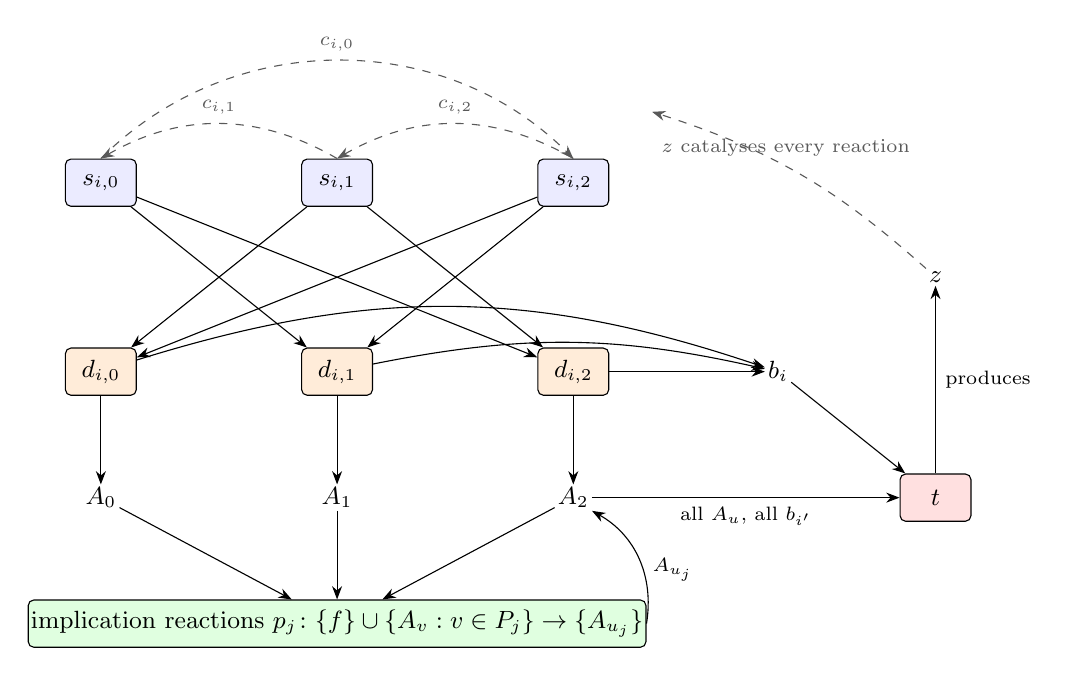
\begin{tikzpicture}[>=Stealth,font=\small,
  sel/.style={draw,rounded corners=2pt,fill=blue!8,minimum width=9mm,minimum height=6mm,inner sep=1pt},
  dec/.style={draw,rounded corners=2pt,fill=orange!15,minimum width=9mm,minimum height=6mm,inner sep=1pt},
  rul/.style={draw,rounded corners=2pt,fill=green!12,minimum width=9mm,minimum height=6mm,inner sep=1pt},
  clo/.style={draw,rounded corners=2pt,fill=red!12,minimum width=9mm,minimum height=6mm,inner sep=1pt},
  mol/.style={inner sep=1pt},
  cat/.style={->,dashed,gray!70!black},
  flow/.style={->}]
  % selector cycle for one slot i with m=3
  \node[sel] (s0) at (0,0) {$s_{i,0}$};
  \node[sel] (s1) at (3.0,0) {$s_{i,1}$};
  \node[sel] (s2) at (6.0,0) {$s_{i,2}$};
  % cyclic catalysis c_{i,u+1} -> s_{i,u}, drawn above the row
  \draw[cat] (s1.north) to[bend right=30] node[above,pos=0.5]{\scriptsize $c_{i,1}$} (s0.north);
  \draw[cat] (s2.north) to[bend right=30] node[above,pos=0.5]{\scriptsize $c_{i,2}$} (s1.north);
  \draw[cat] (s0.north) to[bend left=45] node[above,pos=0.5]{\scriptsize $c_{i,0}$} (s2.north);
  % decoders
  \node[dec] (d0) at (0,-2.4) {$d_{i,0}$};
  \node[dec] (d1) at (3.0,-2.4) {$d_{i,1}$};
  \node[dec] (d2) at (6.0,-2.4) {$d_{i,2}$};
  \draw[flow] (s1) -- (d0); \draw[flow] (s2) -- (d0);
  \draw[flow] (s0) -- (d1); \draw[flow] (s2) -- (d1);
  \draw[flow] (s0) -- (d2); \draw[flow] (s1) -- (d2);
  % statements and marker
  \node[mol] (A0) at (0,-4.0) {$A_0$};
  \node[mol] (A1) at (3.0,-4.0) {$A_1$};
  \node[mol] (A2) at (6.0,-4.0) {$A_2$};
  \node[mol] (b) at (8.6,-2.4) {$b_i$};
  \draw[flow] (d0) -- (A0); \draw[flow] (d1) -- (A1); \draw[flow] (d2) -- (A2);
  \draw[flow] (d0) to[bend left=18] (b); \draw[flow] (d1) to[bend left=12] (b); \draw[flow] (d2) -- (b);
  % implication reactions
  \node[rul] (p) at (3.0,-5.6) {implication reactions $p_j\colon \{f\}\cup\{A_v: v\in P_j\}\to\{A_{u_j}\}$};
  \draw[flow] (A0) -- (p); \draw[flow] (A1) -- (p); \draw[flow] (A2) -- (p);
  \draw[flow] (p.east) to[bend right=35] node[right,pos=0.4]{\scriptsize $A_{u_j}$} (A2.south east);
  % closing reaction
  \node[clo] (t) at (10.6,-4.0) {$t$};
  \node[mol] (z) at (10.6,-1.2) {$z$};
  \draw[flow] (b) -- (t);
  \draw[flow] (A2) -- node[below,pos=0.5]{\scriptsize all $A_u$, all $b_{i'}$} (t);
  \draw[flow] (t) -- node[right,pos=0.5]{\scriptsize produces} (z);
  \draw[cat] (z) to[bend right=12] node[above,pos=0.55]{\scriptsize $z$ catalyses every reaction} (7.0,0.9);
\end{tikzpicture}
\caption{One slot of Construction~\ref{con:axiom} for $m=3$. Solid arrows are reactant/product incidences (every selector also consumes the food molecule $f$, not drawn), dashed arrows are catalysis. The selector cycle $I_i=\{s_{i,0},s_{i,1},s_{i,2}\}$ is the listed irrRAF of the slot; the other slots $i'\neq i$ carry further cycles feeding the same closing reaction $t$. Decoder $d_{i,u}$ needs the signals $x_{i,v}$ of all selectors except $s_{i,u}$, so in an unlisted irrRAF, which omits exactly one selector per slot, the decoder that fires names the omitted statement as an axiom.}
\label{fig:slot}
\end{figure}

Each reaction family has one role. Selectors form the listed cycles and emit the signals $x_{i,u}$. Decoders read a slot: $d_{i,u}$ can fire only if every selector of slot $i$ other than $s_{i,u}$ is present, and it announces statement $u$ as an axiom. Implication reactions copy the rules of $\cA$ on statement molecules; the food reactant $f$ in $p_j$ makes empty-premise rules well defined. The closing reaction $t$ verifies that every slot has been decoded and every statement has been derived, and pays for that verification by producing $z$, the only catalyst available to anything but a selector. Three provenance facts are immediate from Table~\ref{tab:construction} and are used repeatedly: $x_{i,u}$ and $c_{i,u}$ are produced only by $s_{i,u}$; $b_i$ is produced only by decoders of slot $i$; $z$ is produced only by $t$.

\begin{example}[a worked instance]\label{ex:worked}
Take $U=\{0,1,2\}$ with the cyclic rules $\{0\}\Rightarrow1$, $\{1\}\Rightarrow2$, $\{2\}\Rightarrow0$ and $k=1$. Any single statement generates $U$, so the instance is a yes-instance. The system $\cQ(\cA)$ has $12$ molecules and $10$ reactions: three selectors, three decoders, three implication reactions and $t$. Enumerating all $2^{10}-1$ nonempty reaction subsets under Definition~\ref{def:raf} finds $33$ RAFs and exactly four irrRAFs: the listed cycle $I_1=\{s_{1,0},s_{1,1},s_{1,2}\}$ and the three unlisted sets
\[
\{s_{1,1},s_{1,2},\,d_{1,0},\,p_0,p_1,\,t\},\quad
\{s_{1,0},s_{1,2},\,d_{1,1},\,p_1,p_2,\,t\},\quad
\{s_{1,0},s_{1,1},\,d_{1,2},\,p_2,p_0,\,t\},
\]
one for each choice of the omitted selector, that is, of the axiom. In each unlisted irrRAF the implication reaction that would close the cycle of rules is absent, as irreducibility demands. With $k=0$ the same rules give a system whose only candidate for the closing reaction is $t\colon\{A_0,A_1,A_2\}\to\{z\}$ with no producer of any $A_u$, and indeed the system has no RAF at all, matching the fact that the empty set generates nothing. With the single rule $\{0\}\Rightarrow1$ instead, the instance needs two axioms: for $k=1$ the only irrRAF is the listed cycle, while for $k=2$ the two unlisted irrRAFs correspond to the slot assignments $(0,2)$ and $(2,0)$.
\end{example}

\section{Correctness of the reduction}\label{sec:correctness}

Throughout this section $\cA$ is a normalized instance, $\cQ=\cQ(\cA)$, $\cL=\cL(\cA)$, and closures are taken in $\cQ$.

\begin{lemma}[guards]\label{lem:guards}
Each $I_i$ is an irrRAF of $\cQ$, the family $\cL$ has exactly $k$ members, and every irrRAF of $\cQ$ that does not contain $t$ is one of the $I_i$.
\end{lemma}

\begin{proof}
Every selector consumes only food, so all products of $I_i$ lie in $K_1(I_i)$; in particular $c_{i,u+1}\in\cl(I_i)$ catalyses $s_{i,u}$, and $I_i$ is a RAF. Let $H\subseteq I_i$ be a nonempty RAF. Since $t\notin H$ and $t$ is the only producer of $z$, we have $z\notin\cl(H)$, so each $s_{i,u}\in H$ must be catalysed by $c_{i,u+1}\in\cl(H)$, whose only producer is $s_{i,u+1}$; hence $s_{i,u+1}\in H$. Following the cyclic successor around the $m$-cycle from any member of $H$ gives $H=I_i$. Thus $I_i$ is irreducible. The sets $I_i$ are pairwise disjoint and nonempty, so $|\cL|=k$.

Now let $J$ be an irrRAF with $t\notin J$. Then $z\notin\cl(J)$, and since every non-selector reaction has $z$ as its only catalyst, $J$ consists of selectors. Take $s_{i,u}\in J$; the successor argument above, applied to $J$, shows $I_i\subseteq J$, and irreducibility of $J$ together with $I_i$ being a RAF gives $J=I_i$.
\end{proof}

\begin{lemma}[omission pattern]\label{lem:omission}
Let $J$ be an irrRAF of $\cQ$ with $J\notin\cL$. Then $t\in J$; for every slot $i$ there is a unique $a(i)\in U$ such that
\[
s_{i,u}\in J\iff u\neq a(i)\qquad(u\in U);
\]
and every decoder $d_{i,u}\in J$ has $u=a(i)$.
\end{lemma}

\begin{proof}
By Lemma~\ref{lem:guards}, $t\in J$. Fix a slot $i$. Since $I_i$ is a RAF and $J$ is irreducible with $J\ne I_i$, we have $I_i\not\subseteq J$: some selector of slot $i$ is missing from $J$. On the other hand $t\in J$ is food-generated, so $b_i\in\cl(J)$, and $b_i$ is produced only by decoders of slot $i$; hence some $d_{i,u}\in J$. This decoder is food-generated, so $x_{i,v}\in\cl(J)$ for every $v\ne u$, and $x_{i,v}$ is produced only by $s_{i,v}$; hence $s_{i,v}\in J$ for all $v\ne u$. Thus at most one selector of slot $i$ is missing, and combined with the first observation exactly one is: call it $s_{i,a(i)}$, so that $u=a(i)$ for the decoder just considered. Finally, any decoder $d_{i,u'}\in J$ with $u'\ne a(i)$ would need $x_{i,a(i)}\in\cl(J)$, whose only producer $s_{i,a(i)}$ is absent from $J$; this contradicts food generation. For $k=0$ the slot statements are vacuous and only $t\in J$ is asserted.
\end{proof}

All three arguments track the \emph{producer} of a molecule that appears in a staged closure, not merely the set of reactions that list it as a product. This is what prevents a signal produced by an unrelated reaction from being misread as a chosen axiom, and it is why no acyclicity assumption on the implication system is needed.

\begin{theorem}[reduction correctness]\label{thm:correct}
$\cA$ has a generating set of size at most $k$ if and only if $\Extra(\cQ(\cA),\cL(\cA))$ holds. In words: the source instance is a yes-instance if and only if the supplied family is incomplete.
\end{theorem}

\begin{proof}
\emph{Forward direction.} By Lemma~\ref{lem:slots} choose a slot assignment $a$ with $B(a)$ generating $U$. Let
\[
S(a)=\{s_{i,u}: u\ne a(i)\}\cup\{d_{i,a(i)}: i\in[k]\}\cup\{p_j: j<q\}\cup\{t\}.
\]
We show that $S(a)$ is a RAF. Food generation: selectors consume only $f$. Every reactant $x_{i,v}$, $v\ne a(i)$, of the decoder $d_{i,a(i)}$ is produced at stage~$1$ by $s_{i,v}\in S(a)$, so the decoders fire at stage~$2$ and produce every $b_i$ and every $A_{a(i)}$. We claim that every derivable statement $u$ has $A_u\in\cl(S(a))$; by induction on a derivation of $u$ from $B(a)$: if $u\in B(a)$ then $u=a(i)$ for some $i$ and $A_u\in K_2(S(a))$; if $u=u_j$ is obtained by rule $j$ from premises in $P_j$, then by induction each $A_v$, $v\in P_j$, lies in some stage, and since stages increase they all lie in a common stage $K_s(S(a))$, together with $f$, so $p_j$ fires and $A_{u_j}\in K_{s+1}(S(a))$. As $B(a)$ generates $U$, every $A_u$ lies in $\cl(S(a))$. Hence every $p_j$ is food-generated, all reactants of $t$ are in $\cl(S(a))$, $t$ fires, and $z\in\cl(S(a))$. Reflexive autocatalysis: $z$ catalyses every reaction. So $S(a)$ is a nonempty RAF. Let $J\subseteq S(a)$ be an inclusion-minimal RAF (Lemma~\ref{lem:one-deletion}). For each $i$, $s_{i,a(i)}\notin S(a)\supseteq J$, so $J\ne I_i$; thus $J$ is an unlisted irrRAF.

\emph{Reverse direction.} Let $J$ be an unlisted irrRAF and let $a$ be the assignment of Lemma~\ref{lem:omission}. We prove by induction on the stage $h$ that
\[
A_u\in K_h(J)\ \Longrightarrow\ u \text{ is derivable from } B(a).
\]
For $h=0$, $K_0(J)=\{f\}$ contains no statement molecule. For the step, suppose $A_u\in K_{h+1}(J)\setminus K_h(J)$. Then $A_u$ is a product of some reaction $r\in J$ whose reactants lie in $K_h(J)$. Selectors and $t$ produce no statement molecules. If $r=d_{i,u}$ then $u=a(i)\in B(a)$ by Lemma~\ref{lem:omission}. If $r=p_j$ then $u=u_j$ and $A_v\in K_h(J)$ for every $v\in P_j$; by the induction hypothesis each such $v$ is derivable from $B(a)$, and rule $j$ derives $u_j$. This exhausts the reaction types. Since $t\in J$ is food-generated, every $A_u$ lies in some $K_h(J)$, so every statement is derivable from $B(a)$, a set of size at most $k$.
\end{proof}

Cyclic rules do not create unsupported derivations in the reverse direction: a statement molecule enters the closure at a definite first stage through a decoder, which names an axiom, or through an implication whose premises entered earlier. Nor does the order of catalyst appearance matter: $z$ appears only after $t$ fires, which is after all statement molecules are present, and Remark~\ref{rem:semantics} is exactly what permits this.

\section{Size, construction time and the classification}\label{sec:classification}

\begin{proposition}[size]\label{prop:size}
$\cQ(\cA)$ has exactly $M=2+2km+k+m$ molecules and $H=2km+q+1$ reactions. A dense Boolean encoding consisting of a food-membership vector, three molecule-by-reaction incidence matrices (reactants, products, catalysis) and $k$ reaction-membership rows for the listed family has exactly $E=M+(3M+k)H$ cells. The supplied family has exactly $k$ distinct members, all irrRAFs.
\end{proposition}

\begin{proof}
Count Table~\ref{tab:construction}; the last sentence is Lemma~\ref{lem:guards}. The three identities are also Lean theorems (Section~\ref{sec:verification}).
\end{proof}

\begin{proposition}[construction time]\label{prop:time}
The map $\cA\mapsto(\cQ(\cA),\cL(\cA))$ is computable in time polynomial in $k+m+q+L_\cA$, where $L_\cA$ is the encoded length of the rule lists. On classically normalized inputs ($k\le m$) this is polynomial in the input length; on arbitrary inputs it is bounded by a computable function of $k$ times a polynomial in the input length, and the output parameter equals $k$.
\end{proposition}

\begin{proof}
Enumerate the index sets of Table~\ref{tab:construction} and decide each of the $E=O\bigl((km+m)(km+q)\bigr)$ cells of the dense encoding directly from the defining formulas: membership of $x$ in $\inn(r)$, $\out(r)$ or as a catalyst of $r$ is a constant number of index comparisons, one cyclic successor computation, or a scan of one premise list $P_j$ of length at most $L_\cA$. Headers and index names add polynomial overhead. No closure computation, no search for a generating set, and no RAF computation is performed. The parameter claim is Proposition~\ref{prop:size}. Dimension headers may be written in unary so that $k$ contributes at most polynomially to the output length.
\end{proof}

\begin{theorem}[classification]\label{thm:main}
\leavevmode
\begin{enumerate}[label=\textup{(\roman*)}]
\item \Extra{} restricted to valid inputs is $\NP$-complete, and \Exact{} is $\coNP$-complete.
\item Parameterized by $k=|\cL|$, \Extra{} restricted to valid inputs is $\WP$-complete and \Exact{} is $\coWP$-complete.
\item Hardness in \textup{(i)} and \textup{(ii)} holds on inputs $(\cQ,\cL)$ in which $\cQ$ has one food molecule, $\cL$ consists of exactly $k$ pairwise reaction-disjoint irrRAFs each of which is a simple catalytic cycle of reactions with the single reactant $f$ and two catalysts, and every other reaction has a single catalyst $z$.
\end{enumerate}
\end{theorem}

\begin{proof}
Upper bounds are Proposition~\ref{prop:membership}. For the lower bounds compose the normalization of Section~\ref{sec:source-norm} with Construction~\ref{con:axiom}. By Theorem~\ref{thm:correct} the map sends yes-instances of \MAS{} to instances satisfying \Extra{} and no-instances to instances satisfying $\Complete$; all outputs satisfy \Valid{} by Lemma~\ref{lem:guards}, so \Extra{} and $\neg\Exact$ coincide on them. By Proposition~\ref{prop:time} the map is a polynomial-time many-one reduction on classically normalized inputs, giving $\NP$-hardness of \Extra{} on valid inputs from the $\NP$-completeness of \MAS; and it is an FPT reduction with output parameter exactly $k$, giving $\WP$-hardness from~\cite[Theorem~3.3]{abrahamson1995completeness}. Taking complements, \Exact{} is $\coNP$-hard and $\coWP$-hard, already on valid inputs. The restrictions in (iii) are read off Table~\ref{tab:construction}: the listed sets are the pairwise disjoint cycles $I_i$, each selector has reactant set $\{f\}$ and catalysts $c_{i,u+1}$ and $z$, and every other reaction is catalysed only by $z$.
\end{proof}

\begin{remark}[what is and is not restricted]
Reactant arity is unbounded in the hard instances: decoders have $m-1$ reactants and the closing reaction has $k+m$. The implication subsystem may contain cycles. We make no bounded-arity or acyclic-verifier hardness claim; see Section~\ref{sec:discussion}. The listed irrRAFs all have size $m$, which is unbounded, as Proposition~\ref{prop:fpt-boundary} requires.
\end{remark}

\section{Consequences and boundaries}\label{sec:consequences}

\subsection{Reading the classification}

Table~\ref{tab:reading} states what each established claim licenses. Here $\Nlen$ is the full encoded input length and $\FPT\neq\WP$, $\Ptime\neq\NP$ and $\ETH$ are the respective standard assumptions. The distinction between $\XP$ and $\FPT$ is the whole content of the 2013 question: fixing the number of listed sets leaves a polynomial whose degree grows with that number, whereas fixed-parameter tractability demands a degree independent of it.

\begin{table}[t]
\centering
\small
\begin{tabular}{@{}>{\raggedright\arraybackslash}p{0.40\textwidth}>{\raggedright\arraybackslash}p{0.54\textwidth}@{}}
\toprule
\textbf{Established claim} & \textbf{Appropriate interpretation}\\
\midrule
\Exact{} is $\coNP$-complete (Thm.~\ref{thm:main}) & A polynomial-time completeness test for general systems would imply $\Ptime=\NP$.\\
\Exact{} is $\coWP$-complete in $k$ (Thm.~\ref{thm:main}) & A test running in time $f(k)\,\Nlen^{c}$ with $c$ independent of $k$ would imply $\FPT=\WP$; this answers the question of~\cite{steel2013minimal} negatively under that assumption.\\
No $f(k)\,\Nlen^{o(k)}$ algorithm under $\ETH$ (Cor.~\ref{cor:eth}) & The linear dependence of the exponent on $k$ in the deletion procedure cannot be improved to sublinear.\\
$\FPT$ in $k+\ell$ (Prop.~\ref{prop:fpt-boundary}) & When the listed irrRAFs are small, completeness is tractable for moderately many of them.\\
Polynomial verification of an unlisted irrRAF (Lemma~\ref{lem:one-deletion}) & A discovered missing member can be checked efficiently; this is not an efficient certificate that none exists.\\
Exact test in $\XP$ (Lemma~\ref{lem:transversal}) & Exhaustiveness is decidable, and practical for small $k$, even though the worst-case running time is large.\\
\bottomrule
\end{tabular}
\caption{Interpretation of the results at the strength proved.}
\label{tab:reading}
\end{table}

We do not infer a counting classification (no counting reduction is given), average-case hardness (the results are worst-case), or any statement about kinetic persistence or thermodynamic feasibility (the results concern the combinatorial RAF condition only).

\subsection{An exponent lower bound under ETH}\label{sec:eth}

$\WP$-hardness by itself yields no quantitative lower bound on the exponent. A second reduction, from $k$-\Clique, does. It predates the \MAS{} reduction in our development, uses the same selector cycles and closing reaction, and is included in the Lean development (Section~\ref{sec:verification}); we describe it and give the proof in outline, since its two decisive lemmas are the same as Lemmas~\ref{lem:guards} and~\ref{lem:omission}.

\begin{construction}[clique guards]\label{con:clique}
Let $G$ be a simple graph on the vertex set $V=\{0,\dots,n-1\}$, $n\ge2$, and let $k\ge0$. Put $W=[k]\times V$ and call an ordered pair $e=((i,u),(j,v))\in W\times W$ \emph{forbidden} if $i\ne j$ and $uv\notin E(G)$; in particular two copies of the same vertex in different slots form a forbidden pair. The CRS $\cQ(G,k)$ has food $\{f\}$; molecules $f$, $x_w,c_w$ $(w\in W)$, $b_i$ $(i\in[k])$, $y_e$ $(e\in W\times W)$ and $z$; and the reactions below, where $v+1$ is taken modulo $n$:
\begin{align*}
s_{i,v}&\colon \{f\}\to\{x_{i,v},c_{i,v}\}, &&\text{catalysts } c_{i,v+1} \text{ and } z,\\
d_{i,v}&\colon \{x_{i,w}: w\in V,\ w\ne v\}\to\{b_i\}, &&\text{catalyst } z,\\
l_e,\ r_e&\colon \{x_{e_1}\}\to\{y_e\}\ \text{ and }\ \{x_{e_2}\}\to\{y_e\} \text{ if $e$ is forbidden}, &&\text{catalyst } z,\\
l_e,\ r_e&\colon \{f\}\to\{y_e\}\ \text{ (both) if $e$ is not forbidden}, &&\text{catalyst } z,\\
t&\colon \{b_i: i\in[k]\}\cup\{y_e: e\in W\times W\}\to\{z\}, &&\text{catalyst } z.
\end{align*}
The supplied family is $\{I_1,\dots,I_k\}$ with $I_i=\{s_{i,v}: v\in V\}$.
\end{construction}

\begin{proposition}\label{prop:clique}
$G$ has a clique of size $k$ if and only if $\Extra(\cQ(G,k),\{I_1,\dots,I_k\})$ holds. The family is valid with exactly $k$ members, and $\cQ(G,k)$ has $2+2kn+k+(kn)^2$ molecules and $2kn+2(kn)^2+1$ reactions.
\end{proposition}

\begin{proof}[Proof outline]
Lemmas~\ref{lem:guards} and~\ref{lem:omission} hold verbatim, with the pair gates in the role of the implication reactions: they produce no signal, no cyclic catalyst, no marker and no $z$. Let $J$ be an unlisted irrRAF with omission assignment $a\colon[k]\to V$. Since $t\in J$ is food-generated, every $y_e$ is in $\cl(J)$. For a forbidden pair $e=((i,u),(j,v))$ this requires $x_{i,u}$ or $x_{j,v}$ in $\cl(J)$, i.e.\ $u\ne a(i)$ or $v\ne a(j)$. Hence $a(i)a(j)\in E(G)$ for all $i\ne j$, and $a$ is injective because equal vertices in distinct slots are forbidden; so $a([k])$ is a $k$-clique. Conversely, given a $k$-clique $\{a(1),\dots,a(k)\}$, the set consisting of all selectors $s_{i,v}$ with $v\ne a(i)$, the decoders $d_{i,a(i)}$, for each pair $e$ the gates among $l_e,r_e$ whose reactant is available, and $t$, is a RAF, and an inclusion-minimal RAF inside it is unlisted. The counts are read off the construction.
\end{proof}

\begin{corollary}[ETH lower bound]\label{cor:eth}
Unless $\ETH$ fails, there is no algorithm deciding \Exact{} in time $f(k)\,\Nlen^{o(k)}$ for any computable $f$, even on inputs of the restricted form of Theorem~\ref{thm:main}\textup{(iii)}.
\end{corollary}

\begin{proof}
Given $(G,k)$ with $n\ge2$ vertices, Construction~\ref{con:clique} is computable in time polynomial in $k$ and $n$, its output parameter is $k$, and by Proposition~\ref{prop:clique} its dense encoding has length $\Nlen\le c_0\,k^4n^4$ for a constant $c_0$. Suppose \Exact{} were decidable in time $f(k)\,\Nlen^{h(k)}$ with $h(k)=o(k)$. Composing, $k$-\Clique{} would be decidable in time $(kn)^{O(1)}+f(k)\,(c_0k^4n^4)^{h(k)}=f_1(k)\,n^{4h(k)+O(1)}=f_1(k)\,n^{o(k)}$, contradicting~\cite{chen2006strong}. The restricted form holds because $\cQ(G,k)$ has the same guard structure as $\cQ(\cA)$.
\end{proof}

\subsection{Finding one more irrRAF, and enumeration with bounded delay}

Consider the search problem \textsc{Another-irrRAF}: given $\cQ$ and a valid family $\cL$, return an irrRAF not in $\cL$ or report correctly that none exists. Any algorithm for it decides \Extra{} on valid inputs, so by Theorem~\ref{thm:main} a polynomial-time algorithm would imply $\Ptime=\NP$, and an $f(k)\,\Nlen^{O(1)}$-time algorithm would imply $\FPT=\WP$. Moreover, the reverse direction of Theorem~\ref{thm:correct} is constructive: from any returned irrRAF the omitted selectors read off a generating axiom set of the source instance.

\begin{corollary}[bounded-delay enumeration]\label{cor:delay}
Suppose an algorithm enumerates, for every CRS $\cQ$, all irrRAFs of $\cQ$ without repetition, and that the delay before its first output, between consecutive outputs, and between its last output and its termination announcement is bounded by a polynomial $p(\Nlen)$. Then $\Ptime=\NP$. If instead the delay after $j$ outputs (including $j=0$ and the termination announcement) is bounded by $f(j)\,\Nlen^{c}$ for a computable $f$ and constant $c$, then $\FPT=\WP$.
\end{corollary}

\begin{proof}
Given $(\cQ,\cL)$, test validity in polynomial time and reject if it fails. Otherwise run the enumerator, comparing each output with $\cL$, and stop at the first unlisted output (answer: incomplete) or at termination (answer: complete). On a valid list at most $k$ listed outputs can precede the stopping event, so at most $k+1$ delays elapse, for a total time of $(k+1)\,p(\Nlen)\,\Nlen^{O(1)}$ in the first case, which is polynomial since $k\le\Nlen$, and $\bigl(\sum_{j\le k}f(j)\bigr)\Nlen^{O(1)}$ in the second. Theorem~\ref{thm:main} gives the conclusions.
\end{proof}

The corollary concerns delay bounds only. It does not exclude enumeration in total time polynomial in the input plus the entire output (output-polynomial enumeration), because the output may be exponentially larger than $\cL$; that question remains open, and by~\cite{minraf2026} it is at least as hard as hypergraph dualization.

\subsection{The positive boundary}

\begin{proposition}[FPT in $k+\ell$]\label{prop:fpt-boundary}
Let $\ell=\max_{I\in\cL}|I|$ (with $\ell=1$ if $\cL=\varnothing$). \Exact{} is decidable in time $\ell^{k}\,\Nlen^{O(1)}$, hence fixed-parameter tractable in the combined parameter $k+\ell$.
\end{proposition}

\begin{proof}
Lemma~\ref{lem:transversal} with the maxRAF oracle, after a polynomial validity test.
\end{proof}

The hard instances of Theorem~\ref{thm:main} have $\ell=m$ unbounded, so the two results are consistent, and $\ell$ is the parameter that separates them. By contrast, structural parameters of the family alone do not help. In the hard instances the listed irrRAFs are pairwise disjoint: the overlap graph of $\cL$ is edgeless, its treewidth and feedback vertex number are zero, and every reaction lies in at most one listed set. Restricting \Exact{} to any constant value of these parameters therefore leaves the problem $\coNP$-hard and, in $k$, $\coWP$-hard. The number of connected components of the overlap graph is $k$ itself in these instances, so hardness at a fixed number of components is not established by them.

\section{Formal verification and computation}\label{sec:verification}

\subsection{Lean formalization}

The finite combinatorial content of Sections~\ref{sec:upper}--\ref{sec:classification} and of Construction~\ref{con:clique} has been formalized in Lean~4 (toolchain \lean{leanprover/lean4:v4.30.0}) over a frozen Mathlib manifest. The RAF semantics is the staged closure and the RAF predicate of Definition~\ref{def:raf}, shared with the other formal developments of this programme. The publication-facing module is \lean{proofs/AllIrrRAFCert/Publication.lean}; its two exact-certification theorems, quoted here verbatim, quantify over an arbitrary finite implication system \lean{A : System n q} on the statement universe \lean{Fin (n+2)} with \lean{q} rules and over an arbitrary decidable simple graph on \lean{Fin (n+2)}, for every number \lean{k} of slots including \lean{k = 0}.

\begin{small}
\begin{verbatim}
theorem axiom_iff_not_exactCertification {k n q : Nat}
    (A : WPHardness.System n q) :
    WPHardness.SmallGenerating A k <->
      not ExactIrrRAFCertification (WPHardness.crs A) WPHardness.cat
        (WPHardness.listedFamily k n q)

theorem clique_iff_not_exactCertification {k n : Nat}
    (G : SimpleGraph (Fin (n+2))) [DecidableRel G.Adj] :
    (exists s : Finset (Fin (n+2)), G.IsNClique k s) <->
      not ExactIrrRAFCertification (crs (graphBad G)) cat
        (listedFamily k n)
\end{verbatim}
\end{small}
\noindent (The Unicode connectives of the source are transliterated here.)



\noindent Here \lean{ExactIrrRAFCertification Q C L} is the conjunction of \lean{ValidListedFamily Q C L} (every member of \lean{L} is an irrRAF) and \lean{AllCertified Q C L} (every irrRAF is in \lean{L}), exactly as in Section~\ref{sec:problems}; \lean{SmallGenerating A k} asserts the existence of a finite set \lean{B} with \lean{B.card <= k} from which every statement is derivable under the inductively defined derivability relation; and \lean{crs}, \lean{cat} and \lean{listedFamily} are the literal finite data of Constructions~\ref{con:axiom} and~\ref{con:clique}. Table~\ref{tab:concordance} maps the statements of this paper to the proof-bearing declarations. The bundled theorem \lean{axiom_reduction} in \lean{Main.lean} additionally records that every listed member is an irrRAF and that the family has exactly \lean{k} members.

\begin{table}[t]
\centering
\small
\begin{tabular}{@{}p{0.40\textwidth}>{\raggedright\arraybackslash}p{0.54\textwidth}@{}}
\toprule
\textbf{Statement in this paper} & \textbf{Lean declaration}\\
\midrule
Lemma~\ref{lem:one-deletion} (one-deletion test) & \lean{AllIrrRAFCert.irrRAF_single_deletion}\\
Lemma~\ref{lem:transversal} (preserving transversal) & \lean{AllIrrRAFCert.extra_iff_preservingTransversal}; image bound \lean{preservingTransversal_card_le}\\
Lemma~\ref{lem:slots} (slots represent small sets) & \lean{WPHardness.smallGenerating_iff_slots}\\
Lemma~\ref{lem:guards} (guards) & \lean{WPHardness.guard_isIrrRAF}, \lean{guards_injective}, \lean{irrRAF_without_close_eq_guard}\\
Lemma~\ref{lem:omission} (omission pattern) & \lean{WPHardness.extra_contains_close}, \lean{extra_omission_pattern}, \lean{decoder_choice}\\
Theorem~\ref{thm:correct}, forward & \lean{WPHardness.derivation_reaches}, \lean{witness_isRAF}, \lean{generating_implies_extra}\\
Theorem~\ref{thm:correct}, reverse (stage induction) & \lean{WPHardness.statement_sound}, \lean{extra_implies_generating}\\
Theorem~\ref{thm:correct}, equivalence & \lean{WPHardness.smallGenerating_iff_extra}; public form \lean{axiom_iff_not_exactCertification}\\
Proposition~\ref{prop:size} (counts, cells, parameter) & \lean{WPHardness.molecule_count}, \lean{reaction_count}, \lean{encoding_card}, \lean{parameter_eq}\\
Dense encoding rows (Prop.~\ref{prop:time}) & \lean{WPHardness.encode} with \lean{encode_food}, \lean{encode_inputs}, \lean{encode_outputs}, \lean{encode_catalysis}, \lean{encode_list}\\
Proposition~\ref{prop:clique} (clique guards) & \lean{Hardness.graph_clique_iff_extra}, \lean{listed_promise}, \lean{parameter_eq}, \lean{encoding_polynomial}; public form \lean{clique_iff_not_exactCertification}\\
\bottomrule
\end{tabular}
\caption{Concordance between the paper and the Lean development. Unqualified names in the middle rows live in the namespace \texttt{AllIrrRAFCert.WPHardness}; the clique row in \texttt{AllIrrRAFCert.Hardness}.}
\label{tab:concordance}
\end{table}

The strict verification bridge compiles the publication module and its $36$ imported dependencies with warnings treated as errors and authenticates the four exported declarations \lean{axiom_iff_not_exactCertification}, \lean{axiom_reduction}, \lean{extra_iff_preservingTransversal} and \lean{clique_iff_not_exactCertification}. The axiom audit of each reports only the standard axioms \lean{propext}, \lean{Classical.choice} and \lean{Quot.sound}; no \lean{sorry} and no custom axiom is admitted. The final successful run took $70$~seconds. The receipt records the SHA-256 digests of the frozen Mathlib manifest (\lean{a8df0b60...bb9fac}), of \lean{Publication.lean} (\lean{15fb4b80...ff3bcdf}) and of every dependency; the full digests are in the reproduction record accompanying the source bundle.

\paragraph{Boundary of the formal claim.} The Lean theorems establish the finite equivalences: for every source instance, a small generating set exists if and only if exact certification fails for the constructed instance, with the listed family valid and of the stated cardinality, and with the stated molecule, reaction and cell counts. They do not formalize Turing machines, complexity classes, the $\WP$-completeness of \MAS, the $\ETH$ lower bound for \Clique, or the polynomial running time of the maxRAF oracle and of the construction. Those are the conventional arguments of Proposition~\ref{prop:membership}, Proposition~\ref{prop:time}, Theorem~\ref{thm:main} and Corollary~\ref{cor:eth}, given in full above. No complexity-theoretic statement is hidden as a Lean axiom.

\subsection{Exhaustive finite checks}

Before formalization, Construction~\ref{con:axiom} was tested against the source predicate on every implication system over two statements: all $256$ subsets of the $8$ possible rules (including empty premises and cycles) for $k\in\{0,1,2\}$, that is $768$ cases, of which $624$ are yes-instances. For each case the listed cycles were confirmed to be irrRAFs and the existence of an unlisted irrRAF, found by a maxRAF-based search, was compared with the existence of a generating slot assignment. No discrepancy was found; the replay takes under a second. An independent script that enumerates all reaction subsets literally under Definition~\ref{def:raf}, with no maxRAF pruning, repeated the $512$ cases with $k\le1$ (finding $368$ yes-instances, which together with the $256$ trivially positive cases for $k=2$ reproduces the count $624$), a random sample of $12$ systems for $k=2$, a random sample of $40$ systems over three statements with $k=1$, and the instances of Examples~\ref{ex:three} and~\ref{ex:worked}, again without discrepancy. Construction~\ref{con:clique} was tested on $4{,}176$ small graph instances and $56$ dense-source cases in the same way. These computations are diagnostics; the universal statements rest on the proofs and the Lean development.

\section{Discussion}\label{sec:discussion}

The 2013 deletion criterion gave an exact completeness test whose exponent grows with the number of listed irrRAFs, and asked whether that growth is necessary. Theorem~\ref{thm:main} says that it is, unless $\FPT=\WP$, and Corollary~\ref{cor:eth} says that it cannot even be made sublinear unless $\ETH$ fails. The certification problem is thereby placed at the top of the $\mathsf{W}$ hierarchy, alongside \MAS{} and \textsc{Weighted Circuit Satisfiability}, rather than at the $\Wone$ level of \Clique. The mechanism is transparent: the listed cycles are rigid, so any additional irrRAF must sacrifice exactly one reaction in each of them, and a system of $k$ such sacrifices is exactly a choice of $k$ axioms. What makes the problem hard is not that there may be exponentially many irrRAFs, but that the omitted reactions of an unknown irrRAF can encode an arbitrary $k$-element choice, and that the closing reaction can check an arbitrary monotone derivation against it.

The results are structural statements about the combinatorial RAF condition. They say nothing about kinetics, thermodynamics, or whether a given irrRAF can actually establish itself from finite copy numbers; those questions require different models. Within the combinatorial setting, several questions remain.

\begin{enumerate}
\item \emph{Bounded arity.} The decoders and the closing reaction of Construction~\ref{con:axiom} have unbounded reactant sets. Is \Exact{} still $\coWP$-hard, or even $\coNP$-hard, when every reaction has at most two reactants? Chaining a decoder through $m-2$ binary intermediate reactions preserves the provenance arguments but introduces new reactions that an unlisted irrRAF might use in unintended ways; we have not verified a bounded-arity variant.
\item \emph{Counting.} Is counting the irrRAFs of a CRS $\#\Ptime$-complete? Theorem~\ref{thm:correct} is not parsimonious: distinct slot assignments with the same axiom set give distinct irrRAFs, and an irrRAF uses only the implication reactions needed for one derivation.
\item \emph{Output-polynomial enumeration.} Corollary~\ref{cor:delay} rules out polynomial delay unless $\Ptime=\NP$. Whether all irrRAFs can be listed in time polynomial in the input and output lengths is open; by~\cite{minraf2026} it is at least as hard as hypergraph dualization, which is not known to be in polynomial time~\cite{fredman1996complexity}.
\item \emph{Structural parameters of the system.} Proposition~\ref{prop:fpt-boundary} identifies the size of the largest listed irrRAF as a parameter that restores tractability. Are there parameters of $\cQ$ itself, such as the treewidth of its reaction graph or the number of catalysts per reaction, under which \Exact{} is fixed-parameter tractable in $k$ plus that parameter? The hard instances have a single catalyst on most reactions and two on the rest, so the catalyst count alone does not suffice.
\end{enumerate}

\subsection*{Data and code availability}

The Lean sources, the verification receipt with all digests, the exhaustive-check scripts and the editable source of this paper are part of the accompanying research workspace and will be made available with the published version.

\bibliographystyle{plain}
\bibliography{refs}

\end{document}
